\subsection{Ý tưởng xây dựng thuật toán}
\label{section:idea}
\subsection{Xây dựng ma trận xác suất ghép cặp ngẫu nhiên $RMP$}

Trong thuật toán MFEA-I thông thường $rmp$ là một giá trị vô hướng biểu diễn chung cho xác suất giao phối ngẫu nhiên giữa các tác vụ, tuy nhiên thực tế thì mỗi cặp tác vụ lại có một mức độ tương quan riêng. Bởi vậy dẫn đến một ý tưởng đó là xây dựng xác suất ghép cặp ngẫu nhiên $rmp$ dưới dạng một ma trận xác suất ghép cặp ngẫu nhiên đối xứng $RMP$ như sau:
\begin{equation}
    RMP =
    \begin{bmatrix}
        rmp_{1,1} & rmp_{1,2} & \cdot & \cdot \\
        rmp_{2,1} & rmp_{2,2} & \cdot & \cdot \\
        \cdot & \cdot & rmp_{j,j} & \cdot \\
        \cdot & \cdot & \cdot & \cdot \\
    \end{bmatrix}
\end{equation}
Trong đó $rmp_{j,k} = rmp_{k,j}$ là hệ số trao đổi giữa tác vụ $j$ và tác vụ $k$, thêm nữa có $rmp_{j,j} = 1$ $\forall j$. 
\subsection{Ước lượng phân phối của các quần thể con}
Tại thời điểm $t$ xem xét phân phối $g^k(x,t)$ là mô hình ước lượng của phân phối chuẩn $p^k(x,t)$ của tác vụ thứ $k$, $g^k(x,t)$ được xây dựng từ tập nhỏ dân số $P^k(t)$. Bằng việc thay thế hàm mật độ của phân phối chuẩn và sử dụng phần tử trong ma trận $RMP$ thay vì giá trị $rmp$ vô hướng ta có phân phối tập con cái được sinh ra như sau:
\begin{equation}
    g_c^k(x,t) = [1 - \frac{0.5}{K}\cdot \sum_{k \neq j}rmp_{k,j}] \cdot g^k(x,t) + \frac{0.5}{K} \sum_{j \neq k} rmp_{k,j} \cdot g^j(x,t).
    \label{equa:true_distribution}
\end{equation}
Với $g_c^k(x,t)$ là mô hình xác suất hỗn hợp ước lượng gần đúng cho quần thể con cái $p_c^k(x,t)$. Như đã trình bày ở trên, để giảm tác động của trao đổi âm giữa các tác vụ thì cần đưa phân phối $p_c(x,t)$ càng gần với phân phối của quần thể $p(x,t)$ càng tốt. Điều này có nghĩa rằng ta học tham số $rmp$ sao cho phân phối hỗn hợp $g_c^k(x,t)$ sao cho nó xấp xỉ với $p^k(x,t)$ trên tập tất cả tác vụ $k \in {1,2,...K}$.

\subsection{Học trực tuyến ma trận RMP}
    \label{sub:rmp-learning}
    Mỗi tác vụ thứ $k$ sẽ tương ứng với một tập cá thể của chúng là $P^k(t)$, tập này tuân theo phân phối $g^k(x,t)$. Và giả sử tại mỗi thế hệ thì trong tập $P^k(t)$ sẽ bao gồm $N/2$ cá thể là cá thể cha mẹ được truyền từ thế hệ trước sang thế hệ này.
    Cùng với đó theo ý tưởng đã trình bày ở phần \ref{section:idea}, ma trận $RMP$ là tham số của mô hình phân phối xác suất hỗn hợp $g_c^k(x,t)$ với $k \in {1,2,...K}$. Một ý tưởng tự nhiên là để $g_c^k(x,t) \approx p^k(x,t)$ thì phân phối $g_c^k(x,t)$ cũng sẽ phù hợp với tập các cá thể của thế hệ hiện tại và các cá thể này sẽ tuân theo phân phối $g_c^k(x,t)$. Vậy bài toán trở thành tối ưu ma trận $RMP$ sao cho cực đại hóa giá trị hàm maximum log-likelihood:
    \begin{equation}
        \max_{RMP}\sum_{k=1}^{K}\sum_{i=1}^{N/2}\log{g_c^k(x_{ik},t)}
        \label{equa:likelihood}
    \end{equation}
    với $x_{ik}$ là cá thể thứ $i$ trong tập $P^k(t)$.
    
    Nhưng liệu khi học ma trận $RMP$ sao cho phân phối $g_c^k(x,t)$ phù hợp với tập các cá thể của thế hệ hiện tại $\forall k \in {1,2,...K}$, thì có kéo theo $g_c^k(x,t)$ trở lên gần với $p^k(x,t)$? Để xác định xem 2 phân phối có thực sự gần nhau hay không thì có một phương pháp thông dụng đó là sử dụng phương pháp phân kỳ Kullback-Leiber (thuật ngữ gốc: \emph{Kullback-Leiber divergence - KL}) \cite{hershey2007approximating}. Một cách cụ thể $KL$ sẽ tính toán lượng thông tin bị mất mát khi hàm mật độ $g$ được sử dụng để ước lượng hàm mật độ $p$. Điều này thể hiện tương đương mức độ gần nhau giữa 2 phân phối.
    Cụ thể $KL$ giữa 2 phân phối $p$ và $g$ được định nghĩa như sau:
    \begin{equation}
        KL(p\Vert g) = \int_{X}p(x)\cdot [log(x) - log(x)]\cdot\,dx
        \label{equa:KL}
    \end{equation}
    Từ suy nghĩ này việc tối ưu sao cho $g_c^k(x,t)$ trở lên gần với $p^k(x,t)$ cũng sẽ tương đương việc tả tối thiểu hóa $KL$ giữa 2 phân phối. Và qua công thức \ref{equa:likelihood} và \ref{equa:KL}, Bali, Ong, Gupta and Tan qua một số biến đổi đơn giản đã chứng minh khi tối đa hóa maximum log-likelihood \ref{equa:likelihood} \cite{white1982maximum} thì cũng sẽ tương đương với việc tối thiểu hóa hàm khoảng cách $KL$ giữa 2 phân phối $p$ và $g$. Hay phân phối $g_c^k(x,t)$ sẽ gần hơn với $p^k(x,t)$ sau quá trình học trực tuyến ma trận $RMP$.
    \begin{equation}
        \text{công thức } \ref{equa:likelihood} \Leftrightarrow \min_{RMP}\sum_{k=1}^{K}KL(p^k(x,t)\|g_c^k(x,t))
        \label{equa:KL}
    \end{equation}
\subsection{Cấu trúc thuật toán}
    Biểu diễn thuật toán qua các bước:
    \begin{figure}[ht]
        \centering
        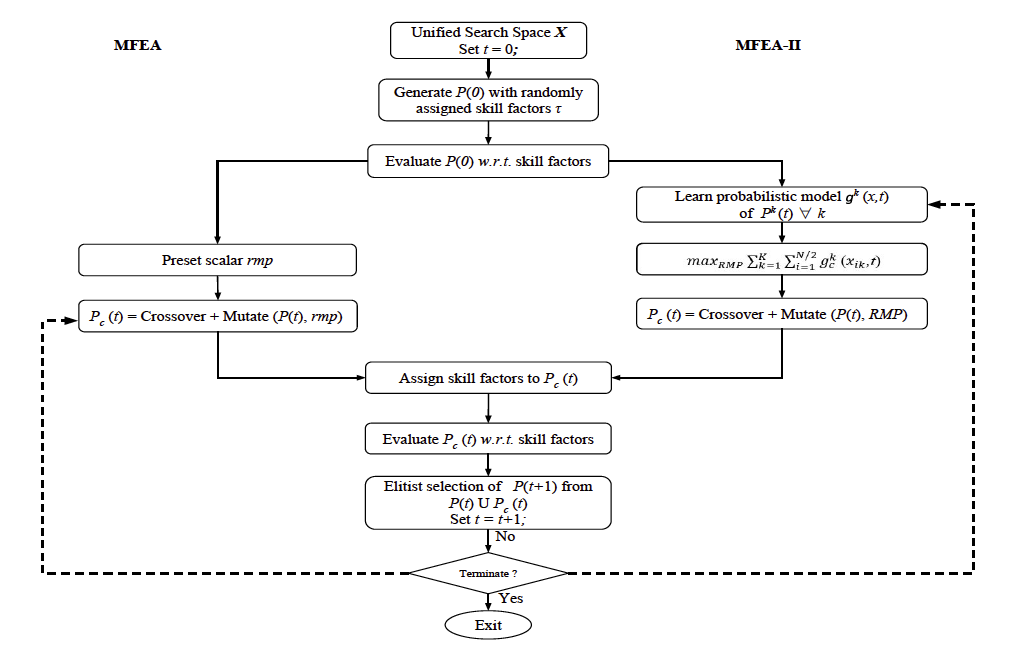
\includegraphics[width=15cm,height=12cm]{mfeaii.png}
        \caption{Lược đồ so sánh các bước thực hiện giải thuật MFEA-I và MFEA-II. Nguồn \cite{bali2019multifactorial}}.
        \label{fig:mfeaii}
    \end{figure}
    Hình \ref{fig:mfeaii} mô tả một góc nhìn tổng quan về sự khác biệt giữa MFEA và MFEA-II. Trong đó có thể chia 2 thuật toán này làm 3 pha chính theo thứ tự từ trên xuống: khởi tạo, trao đổi chéo, đánh giá và lựa chọn. Dễ thấy sự giống nhau nằm ở pha đầu tiên và cuối cùng. Điểm khác biệt của MFEA-II trong phá thứ 2 bởi quá trình học trực tuyến ma trận $RMP$ với phương pháp đã được trình bày ở mục \ref{sub:rmp-learning}. Mô tả quá trình học trực tuyến ma trận $RMP$ dưới dạng mã giả trong thuật toán \ref{alg:online-rmp-learning}
    \begin{algorithm}[ht]
        \caption{Học trực tuyến ma trận $RMP$}
        \begin{algorithmic}[1]
            \State Xây dựng một mô hình phân phối ước lượng $g^k(x,t)$ trên mỗi tập cá thể $P^k(t)$. $\forall k \in {1,2,...K}$
            \State Tối ưu hóa mô hình hỗn hợp $\max_{RMP}\sum_{k=1}^{K}\sum_{i=1}^{N/2}\log{g_c^k(x_{ik},t)}$
        \end{algorithmic}
        \label{alg:online-rmp-learning}
    \end{algorithm} \\
    Pha trao đổi khác tác vụ sẽ được mô tả trong thuật toán 5, khi các giải pháp được trao đổi giữa các tác vụ sẽ phụ thuộc vào ma trận $RMP$ đã học ở thuật toán \ref{alg:inter-task crossover}. Trong trường hợp ma trận $RMP$ học được toàn giá trị $0$ thì MFEA-II sẽ hoạt động tương tự với thuật toán tiến hóa kinh điển trong việc học song song từng tác vụ đơn lẻ. \\ 
    \begin{algorithm}[h!]
        \caption{Trao đổi khác tác vụ trong MFEA-II}
        \begin{algorithmic}[1]
            \State Chọn 2 cá thể ngẫu nhiên $x_i$ và $x_j$ từ quần thể $P(t)$:
            \If {$(\tau_i  \neq \tau_j)$}
                \If {$rand \leq rmp_{\tau_i,\tau_j}$}
                    \State $[x_a, x_b]$ $\leftarrow$ \emph{Trao đổi khác tác vụ} giữa $x_i$ và $x_j$;
                    \State Mỗi cá thể con cái sinh ra sẽ được gán ngẫu nhiên một giá trị thuộc tính kĩ năng $\tau_i$  hoặc $\tau_j$;
                \Else 
                    \State Lựa chọn ngẫu nhiên $x_i^{'}$ với thuộc tính kĩ năng $\tau_i$;
                    \State $[x_a]$ $\leftarrow$ \emph{Trao đổi cùng tác vụ} giữa $x_i$ và $x_i^{'}$;
                    \State Gán cá thể con cái $x_a$ với thuộc tính kĩ năng $\tau_i$;
                    \State Lựa chọn ngẫu nhiên $x_j^{'}$ với thuộc tính kĩ năng $\tau_j$;
                    \State $[x_b]$ $\leftarrow$ \emph{Trao đổi cùng tác vụ} giữa $x_i$ và $x_i^{'}$;
                    \State Gán cá thể con cái $x_b$ với thuộc tính kĩ năng $\tau_j$;
                
        \end{algorithmic}
        \label{alg:inter-task crossover}
    \end{algorithm}
     Tuy nhiên tại sao lại sử dụng MFEA-II để huấn luyện mạng neural trong khi các thuật toán huấn luyện mạng neural kinh điển sử dụng phương pháp gradient-based vẫn đang được hầu hết các nhóm nghiên cứu sử dụng. Trong chương tiếp theo, đồ án sẽ trình bày các yêu cầu cấp thiết của việc áp dụng này và qua đó là đề xuất, giải thuật áp dụng chi tiết.
    